\documentclass[11pt,a4paper,sans]{moderncv}

\moderncvstyle{casual}
\moderncvcolor{blue}

\usepackage[utf8]{inputenc}
\usepackage[T1]{fontenc}
\usepackage[french]{babel}

\usepackage[scale=0.75]{geometry}
\graphicspath{{figures/}}

% personal data
\name{Vincent}{Lafouasse}
\title{Graduate student in Chemistry (M2)}
\address{28 square du clos de Villaine}{91300 Massy}{\textsc{France}}
\phone[mobile]{+33 6 21 59 25 74}
\phone[fixed]{+33 9 50 40 28 82}
\email{vincentlafouasse@live.fr}

%----------------------------------------------------------------------------------
%            content
%----------------------------------------------------------------------------------
\begin{document}

\makecvtitle

%
\section{Research Interest}
\cvitem{\textsc{About me}}{I am mainly interested in the field of Molecular Chemistry, especially Total Synthesis. %
I am currently looking for a 6-month internship beginning January 2021 and am also looking for a PhD for Fall 2021.}

%
\section{Education}
\cventry{Fall 2020}{(M2) M.Sc. in Molecular Chemistry and Interfaces}%
{{\newline}École Normale Supérieure de Paris-Saclay -- École Polytechnique}%
{Paris-Saclay (91)}{}%
{A high-level scientific and academic program devoted to molecular chemistry and its applications to the fields of biology and material sciences. This program gives state-of-the-art knowledge in chemical sciences and brings the students towards their applications in industry.}

%
\cventry{2018--2020}{(M1) M.Sc. in Chemistry}{Université Paris-Sud}{Orsay (91)}{}%
{Organic Chemistry platform}

\cventry{2017--2018}{B.Sc. in Chemistry (Physics minor)}{Sorbonne Université}{Paris (75)}{}%
{Fundamentals of Chemistry and Physics}

\cventry{2015--2017}{B.Sc. Sciences de la Matière}{Ecole Normale Supérieure de Lyon}{Lyon (69)}{}%
{Élève normalien : A unique, non-specialized training program in Physics and Chemistry}

\cventry{2013--2015}{Classe Préparatoires (CPGE) PCSI/PC$^*$}{Lycée Henri IV}{Paris (75)}{}%
{Two years of intensive theoretical courses in Mathematics, Physics and Chemistry in order to prepare for École Normale Supérieure national selective examas well as other prestigious graduate schools.@}

\cventry{2013}{Baccalauréat (A-levels)}{Lycée de l'Île-de-France}{Villebon-sur-Yvette (91)}{}{Science major, Highest Honours}
%

\section{Experience}
%

\subsection{Research}

\cventry{2020}{4 month internship}{ICMMO (UMR 8182)}{Orsay (91)}{Electrocatalysis and CO$_2$ valorization}%
{Under the direction of Mohamed Mellah and Emmanuelle Schulz\newline{}%
Préparation de dérivés de type acide 2-phénylpropanoïque énantioenrichis, en partant d'halogénures benzéniques secondaires par activation du CO2 en présence de quantités catalytiques de Sm(II) électrogénéré
}


\cventry{2018}{Lab week}{Sorbonne Université}{Paris (75)}{Supramolecular Chemistry}%
{Under the direction of Matthieu Sollogoub (IPCM, GOBS) as part of the UE 3C015 TEOREM\newline{}%
Detailed achievements:%
\begin{itemize}%
\item Study of $\beta$-CD based inclusion compounds
\item Synthesis and RMN caracterisation of a $\alpha$-CD based [3]-rotaxane
\item Synthesis and RMN caracterisation of a self-assembled iron cage
\end{itemize}
}

\cventry{2014-2015}{TIPE}{Lycée Henri IV}{Paris (75)}{Supramolecular Chemistry}%
{Under the direction of Julien Lalande \newline{}%
Detailed achievements:%
\begin{itemize}%
\item Synthesis of dibenzo-18-crown-6 using Pedersen's original protocol
\item Qualitative and quantitative study of crown ether complexes with different cations
\end{itemize}
}


\subsection{Teaching}
\cventry{2018--now}{Chemistry Professor}{Optimal Sup Spé}{Paris (75)}{}%
{Teaching groups of CPGE students from all scientific tracks (PC, MP, PSI, BCPST)\newline{}%
Detailed achievements:%
\begin{itemize}%
\item +12h of formation and +200 h of class
\item a lot of {\LaTeX} $~$edition
\item Preparation of students for the national entrance exams to XENS
\end{itemize}
}


\section{Languages}
\cvitemwithcomment{French}{Fluent}{Native speaker}
\cvitemwithcomment{English}{Fluent}{C2 BULATS 05/18}


\section{Skills}
\cvitem{Molecular Chemistry}{Organic Synthesis, Total Synthesis, Supramolecular Chemistry }
\cvitem{General Chem}{Quantum Chemistry, Spectroscopy, Cristallography }
\cvitem{Physics}{Quantum Mechanics, Thermodynamics }
\cvitemwithcomment{Code}%
{Python
\includegraphics[height=1.4\fontcharht\font`\B]{python_logo.png}, %
{\LaTeX}, %
Julia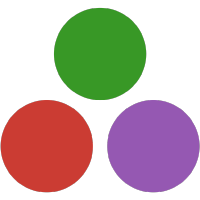
\includegraphics[height=1.4\fontcharht\font`\B]{julia_logo.png}%
}{Familiar}
\cvitemwithcomment{}{C}{Basics}

\section{Interests}
\cvitem{Music}{Jazz guitar, Trumpet}
\cvitem{}{Music theory and Jazz harmony}
\cvitem{}{Dance}



\clearpage

\end{document}
